\section{Double Tuned Mass Damper}
In previous section, we investigated the simplest form of tuned mass damper, which is a mass connected with a spring and a damper. The optimized results were pretty promising. We can dig further into tuned mass dampers by using two masses instead of one. We have a similar constraint as before, which is $m_2+m_3 \leq 0.1\,kg$. Two configurations of double tuned mass dampers (DTMD) are investigated following sections.
\subsection{Parallel Double Tuned Mass Damper}
\begin{figure}[ht]
    \centering
    \documentclass[border=5pt,tikz]{standalone}
\usepackage{tikz}
\usetikzlibrary{calc,patterns,decorations.pathmorphing,decorations.markings}

\begin{document}

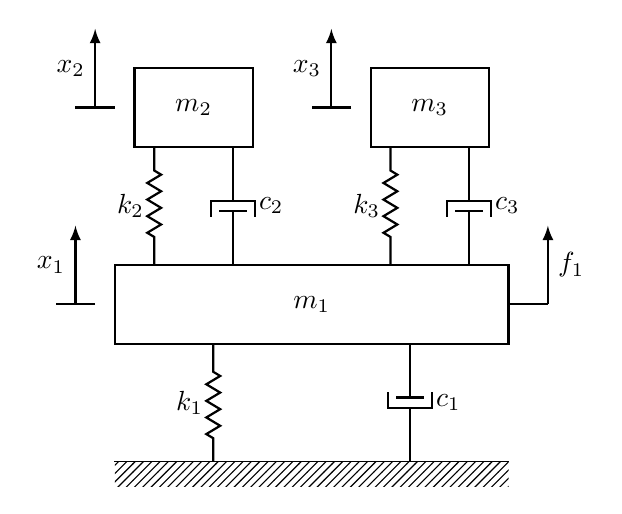
\begin{tikzpicture}
% TikZ Styles
\tikzstyle{mass}=[draw,outer sep=0pt,thick]
\tikzstyle{spring}=[thick,decorate,decoration={zigzag,pre length=0.3cm,post length=0.3cm,segment length=6}]
\tikzstyle{damper}=[thick,decoration={markings,  
  mark connection node=dmp,
  mark=at position 0.5 with 
  {
    \node (dmp) [thick,inner sep=0pt,transform shape,rotate=-90,minimum width=15pt,minimum height=3pt,draw=none] {};
    \draw [thick] ($(dmp.north east)+(2pt,0)$) -- (dmp.south east) -- (dmp.south west) -- ($(dmp.north west)+(2pt,0)$);
    \draw [thick] ($(dmp.north)+(0,-5pt)$) -- ($(dmp.north)+(0,5pt)$);
  }
}, decorate]
\tikzstyle{ground}=[fill,pattern=north east lines,draw=none,minimum width=0.75cm,minimum height=0.3cm]
% Actual Drawing
\node (m1) [mass,minimum width=5cm,minimum height=1cm] {$m_1$};
\node (m2) at (m1.north) [mass,yshift=1.5cm,xshift=-1.5cm,anchor=south,minimum width=1.5cm,minimum height=1cm] {$m_2$};
\node (m3) at (m1.north) [mass,yshift=1.5cm,xshift=1.5cm,anchor=south,minimum width=1.5cm,minimum height=1cm] {$m_3$};

\node (ground) at (m1.south) [ground,yshift=-1.5cm,anchor=north,minimum width=5cm] {};
\draw (ground.north west) -- (ground.north east);
\draw [spring] ([xshift=-1.25cm] ground.north) -- ([xshift=-1.25cm] $(m1.south east)!(ground.north)!(m1.south west)$) node[midway, left]{$k_1$};
\draw [damper] ([xshift=1.25cm] ground.north) -- ([xshift=1.25cm] $(m1.south east)!(ground.north)!(m1.south west)$) node[midway, right,xshift=2mm]{$c_1$};
\draw [spring] ([xshift=-0.5cm]m2.south) -- ([xshift=-0.5cm]$(m1.north east)!(m2.south)!(m1.north west)$) node[midway, left]{$k_2$};
\draw [damper] ([xshift=0.5cm]m2.south) -- ([xshift=0.5cm]$(m1.north east)!(m2.south)!(m1.north west)$) node[midway, right,xshift=2mm]{$c_2$};
\draw [spring] ([xshift=-0.5cm]m3.south) -- ([xshift=-0.5cm]$(m1.north east)!(m3.south)!(m1.north west)$) node[midway, left]{$k_3$};
\draw [thick] (m1.east) -- +(0.5cm,0);
\draw [damper] ([xshift=0.5cm]m3.south) -- ([xshift=0.5cm]$(m1.north east)!(m3.south)!(m1.north west)$) node[midway, right,xshift=2mm]{$c_3$};
\draw [-latex,thick] ([xshift=0.5cm]m1.east) -- +(0,1cm) node[midway, right]{$f_1$};
\draw [thick] ([xshift=-0.25cm]m1.west) -- +(-0.5cm,0);
\draw [-latex,thick] ([xshift=-0.5cm]m1.west) -- +(0,1cm) node[midway, left]{$x_1$};
\draw [thick] ([xshift=-0.25cm]m2.west) -- +(-0.5cm,0);
\draw [-latex,thick] ([xshift=-0.5cm]m2.west) -- +(0,1cm) node[midway, left]{$x_2$};
\draw [thick] ([xshift=-0.25cm]m3.west) -- +(-0.5cm,0);
\draw [-latex,thick] ([xshift=-0.5cm]m3.west) -- +(0,1cm) node[midway, left]{$x_3$};
\end{tikzpicture}
\end{document}
    \caption{SDOF System with parallel DTMD}
    \label{fig:pDTMD}
\end{figure}
The first double tuned mass damper (DTMD) configuration is the parallel one. The parallel DTMD configuration can be seen at figure \ref{fig:pDTMD}.
\subsubsection{Analysis}
EOM can be written as:
\begin{center}
$$
\begin{bmatrix}
m_1 & 0 & 0\\
0 & m_2 & 0\\
0 & 0 & m_3
\end{bmatrix}\cdot
\begin{Bmatrix}
\ddot{x_1}\\
\ddot{x_2}\\
\ddot{x_3}
\end{Bmatrix}+
\begin{bmatrix}
c_1+c_2+c_3 & -c_2 & -c_3\\
-c_2 & c_2 & 0\\
-c_3 & 0 & c_3
\end{bmatrix}\cdot
\begin{Bmatrix}
\dot{x_1}\\
\dot{x_2}\\
\dot{x_3}
\end{Bmatrix}+
\begin{bmatrix}
k_1+k_2+k_3 & -k_2 & -k_3\\
-k_2 & k_2 & 0\\
-k_3 & 0 & k_3
\end{bmatrix}\cdot
\begin{Bmatrix}
x_1\\
x_2\\
x_3
\end{Bmatrix} =
\begin{Bmatrix}
f_1\\
0\\
0
\end{Bmatrix}
$$
\end{center}
This equation has the same closed form as STMD. Therefore the equation can be solved using the same method as before.
\subsubsection{Optimization}
There are 6 system parameters for DTMDs which are $m_2$, $m_3$, $k_2$, $k_3$, $c_2$ and $c_3$. However since the total mass added should be less than 0.1 kg, by equating $m_3$ to $0.1\,kg-m_2$, we can decrease the parameter number to 5.
\par
Similar to STMD optimization, we can try to optimize peak value of the vibration amplitude. We can again use a gradient based optimization algorithm. Different from STMD, we can find multiple local optima using gradient based techniques, which are designed to find local extrema. Therefore finding the global optimum requires couple of different initial guesses using the gradient based approach. Therefore, an constrained genetic algorithm is used to find the region where the global optimum lies. Then, the result of the genetic algorithm can be used as an initial guess to the gradient based algorithm to refine the results.
\par
As the result of the optimization we obtained a system with the resonance vibration amplitude of 4.0684 m. The vibration response of the optimized system can be seen at figure \ref{fig:freq_pDTMD}. The optimized DTMD parameters can be seen below:
\begin{align*}
    m2 & = 0.0505 \,kg\\
    m3 & = 0.0495 \,kg\\
    k2 & = 0.0510 \,N/m\\
    k3 & = 0.0343 \,N/m\\
    c2 & = 0.0139 \,N\cdot s/m\\
    c3 & = 0.0093 \,N\cdot s/m
\end{align*}
\begin{figure}
    \centering
    \includegraphics[scale=0.5]{MATLAB Figures/parallel DTMD.png}
    \caption{Frequency response of the peak optimized parallel DTMD}
    \label{fig:freq_pDTMD}
\end{figure}
\newpage
\subsection{Series Double Tuned Mass Damper}
\begin{figure}[ht]
    \centering
    \input{Figures/series_DTMD_fig}
    \caption{\raggedright SDOF System with series DTMD}
    \label{fig:sDTMD}
\end{figure}
The other DTMD configuration we would like to investigate is the masses connected in series. The configuration can be seen at figure \ref{fig:sDTMD}.
\subsubsection{Analysis}
EOM can be written as:
$$
\begin{bmatrix}
m_1 & 0 & 0\\
0 & m_2 & 0\\
0 & 0 & m_3
\end{bmatrix}\cdot
\begin{Bmatrix}
\ddot{x_1}\\
\ddot{x_2}\\
\ddot{x_3}
\end{Bmatrix}+
\begin{bmatrix}
c_1+c_2 & -c_2 & 0\\
-c_2 & c_2+c_3 & -c_3\\
0 & -c_3 & c_3
\end{bmatrix}\cdot
\begin{Bmatrix}
\dot{x_1}\\
\dot{x_2}\\
\dot{x_3}
\end{Bmatrix}+
\begin{bmatrix}
k_1+k_2 & -k_2 & 0\\
-k_2 & k_2+k_3 & -k_3\\
0 & -k_3 & k_3
\end{bmatrix}\cdot
\begin{Bmatrix}
x_1\\
x_2\\
x_3
\end{Bmatrix} =
\begin{Bmatrix}
f_1\\
0\\
0
\end{Bmatrix}
$$
This equation can be solved using the same method used in previous sections.
\subsubsection{Optimization}
Optimizing the series DTMD is mathematically same as the parallel one. Therefore we can use genetic algorithm to find the region of the global optimum and use a gradient based algorithm to find the optimum exactly.\\
\\
\par The optimized TMD parameters and the frequency response can be seen below:
\begin{align*}
    m2 &= 0.0030 \,kg\\
    m3 &= 0.0970 \,kg\\
    k2 &= 0.0981 \,N/m\\
    k3 &= 0.3164 \,N/m\\
    c2 &= 0.0282 \,N\cdot s/m\\
    c3 &= 0.4281 \,N\cdot s/m
\end{align*}
\begin{figure}[ht]
    \centering
    \includegraphics[scale = 0.6]{MATLAB Figures/series DTMD.png}
    \caption{Frequency response of the peak optimized series DTMD}
    \label{fig:freq_sTMD}
\end{figure}